\documentclass[12pt]{article}
\usepackage[utf8]{inputenc}
\usepackage{amsmath, amssymb, amsthm, geometry}
\usepackage{enumitem}
\usepackage{blindtext}
\usepackage{graphicx}
\graphicspath{{./images}}
\usepackage{caption}
\usepackage{float}

\geometry{margin=1in}
\usepackage{mathtools}

% Define theorem-like environments
\theoremstyle{plain}
\newtheorem{theorem}{Theorem}[section]
\newtheorem{lemma}[theorem]{Lemma}
\newtheorem{proposition}[theorem]{Proposition}
\newtheorem{corollary}[theorem]{Corollary}

\theoremstyle{definition}
\newtheorem{definition}[theorem]{Definition}
\newtheorem{assumption}[theorem]{Assumption}

\theoremstyle{remark}
\newtheorem{remark}[theorem]{Remark}

% Additional useful commands
\newcommand{\E}{\mathbb{E}}
\newcommand{\Prob}{\mathbb{P}}
\newcommand{\R}{\mathbb{R}}




\begin{document}
	\title{ECON 8210 - Quantitative Macroeconomics \\ Homework II}
	\author{Mahmut Eymen Akin \\
		University of Pennsylvania \\
		\texttt{meakin@sas.upenn.edu}}
	\date{\today}
	\maketitle
	
	\section*{Question 5}
	
	Note that the model is summarized in the "\texttt{econ8210hw2q1-2\_meakin.ipynb}" file. Figures 1-4 show the consumption, labor, and next period capital stock policy functions computed through associated solution methods. Looking at the Figures 1 and 2, one can easily observe that the policies obtained through Chebyshev Polynomials Projection are more or less the same as those obtained through Finite Elements Projection. Conceptually, we know that Finite Elements Projection is much more precise in terms of approximating the policies. Hence, we can conclude that although it is a rougher tool, using Chebyshev approximation does not lead to any losses in precision for this particular approximation. Moreover, as evident in Figure 3, the policy functions obtained through a 3rd Order Perturbation also yield very similar results. However, looking at Figure 4, one can see that the policy functions computed through Neural Network is a little bit different from the rest. Although the overall behavioral pattern seems to be the same along the capital stock dimension (i.e. as current capital stock increases, next period capital stock increases, labor decreases, and consumption increases), there are some irregularities as well. For example, as capital stock increases, the relative standing of the abor effort exerted across different productivity states change. For higher capital stock levels, agents at the lower productivity state work more and vice versa. Additionally, one can observe sharp increases in consumption policy and and a sharp decrease in labor policy in early levels. However, it is highly likely that these discrepancies are solely due to the differences in the ranges displayed on the x-axes of the graphs. The sudden spike in consumption and the sudden drop in labor occur at capital stock values well below 2, which are not displayed in earlier graphs. Yet, the change in relative standings of labor policies and lower productivity state agents working more are phenomena that occur within the bounds displayed in earlier plots. Lastly, the next period capital policies of the neural net seems to be way less responsive to productivity shocks than the those computed through the other methods. Hence, the neural net seems to struggle when it comes to approximating the policies and may be in need of better tuning. 
	
	Another issue is the computational resources required to conduct each computation. The most computationally demanding method was Finite Elements projection, which roughly took 10 minutes to run. It was followed by the neural net by roughly 5 minutes. The next in line was the Chebyshev Projection, which took roughly 40 seconds. The most efficient method was by far the perturbation, which took less than a second to run. The differences are even more striking, considering the fact that Finite Elements and Chebyshev were written using Julia, a much faster language. The Perturbation was done through Dynare and MATLAB, whereas the neural network were conducted through Python. Hence, the computational demand of the Neural Net may be overstated, as Python is the slowest language compared to the others mentioned above. Yet, even with the computational advantage of Julia, Perturbation performed much better. This may as well be due to poor coding practices, as Perturbation relied on Dynare whereas the Projection methods were coded by the author. Nonetheless, even without such confounding factors, it is unlikely for the relative standing of Projection and Perturbation methods to change. Hence, it is the opinion of the author that it is much more advantageous to use Perturbation. 
	
	\begin{figure}[H]
		\centering
		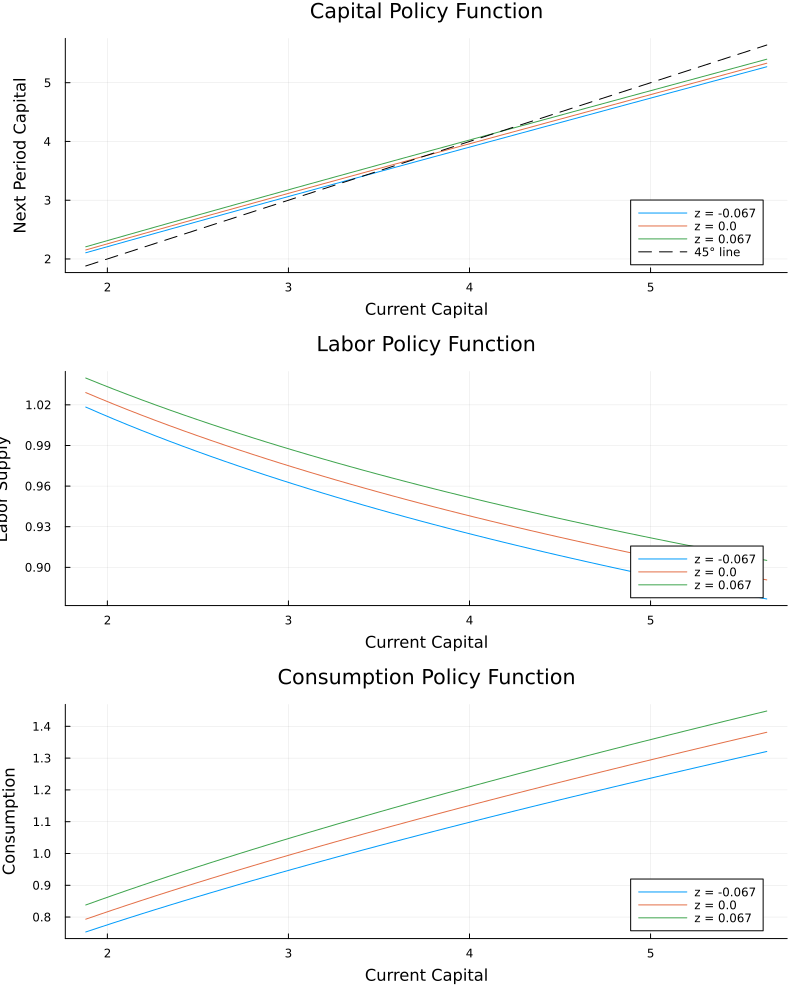
\includegraphics[width=\textwidth]{q1fin.png}
		\caption{Chebyshev Polynomials Projection Policy Functions}
	\end{figure}
	\pagebreak
	
	% Figure 2
	\begin{figure}[H]
		\centering
		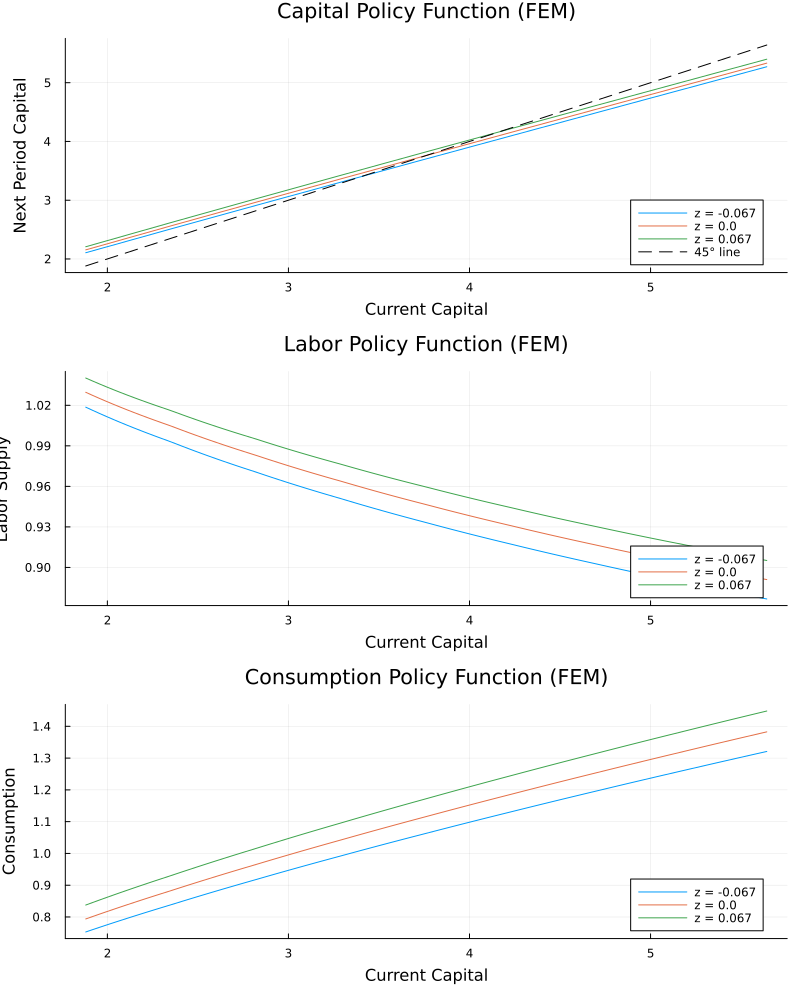
\includegraphics[width=\textwidth]{q2fin.png}
		\caption{Finite Elements Projection Policy Functions}
	\end{figure}
	\pagebreak
	
	% Figure 3
	\begin{figure}[H]
		\centering
		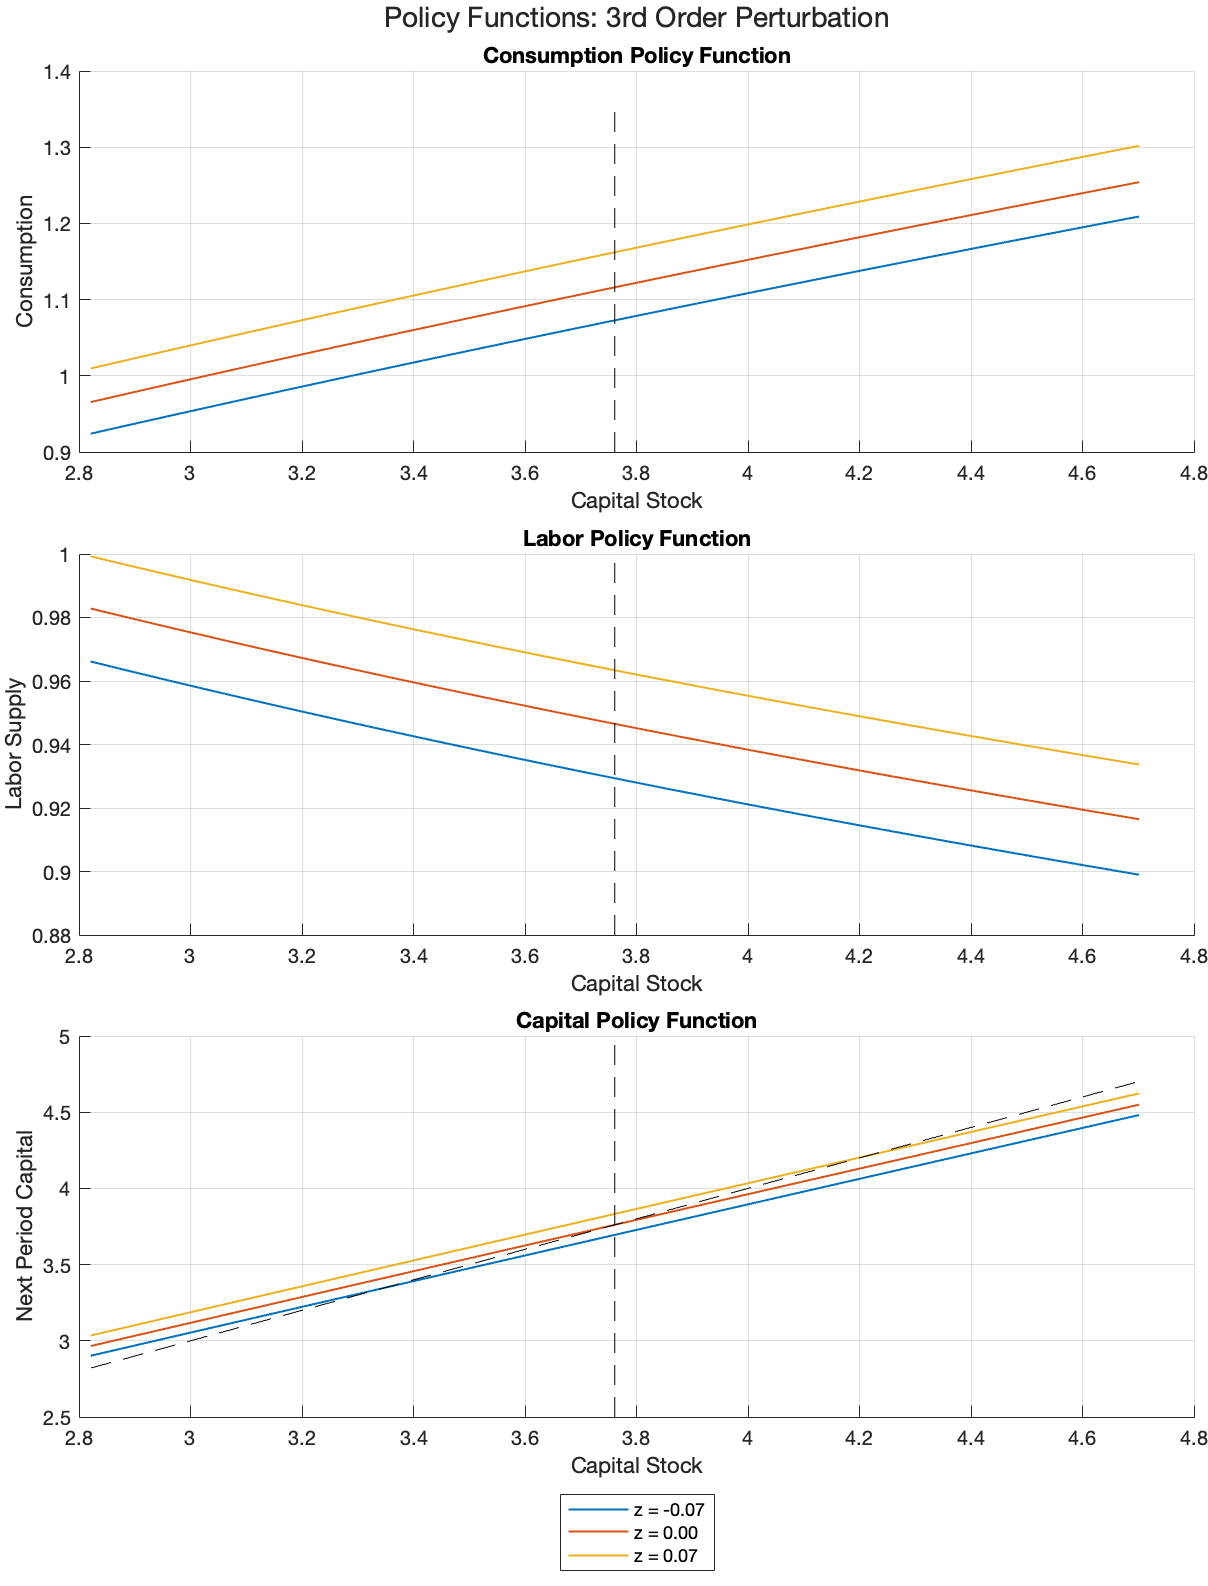
\includegraphics[width=\textwidth]{q3fin.png}
		\caption{3rd Order Perturbation Policy Functions}
	\end{figure}
	\pagebreak
	
	% Figure 4
	\begin{figure}[H]
		\centering
		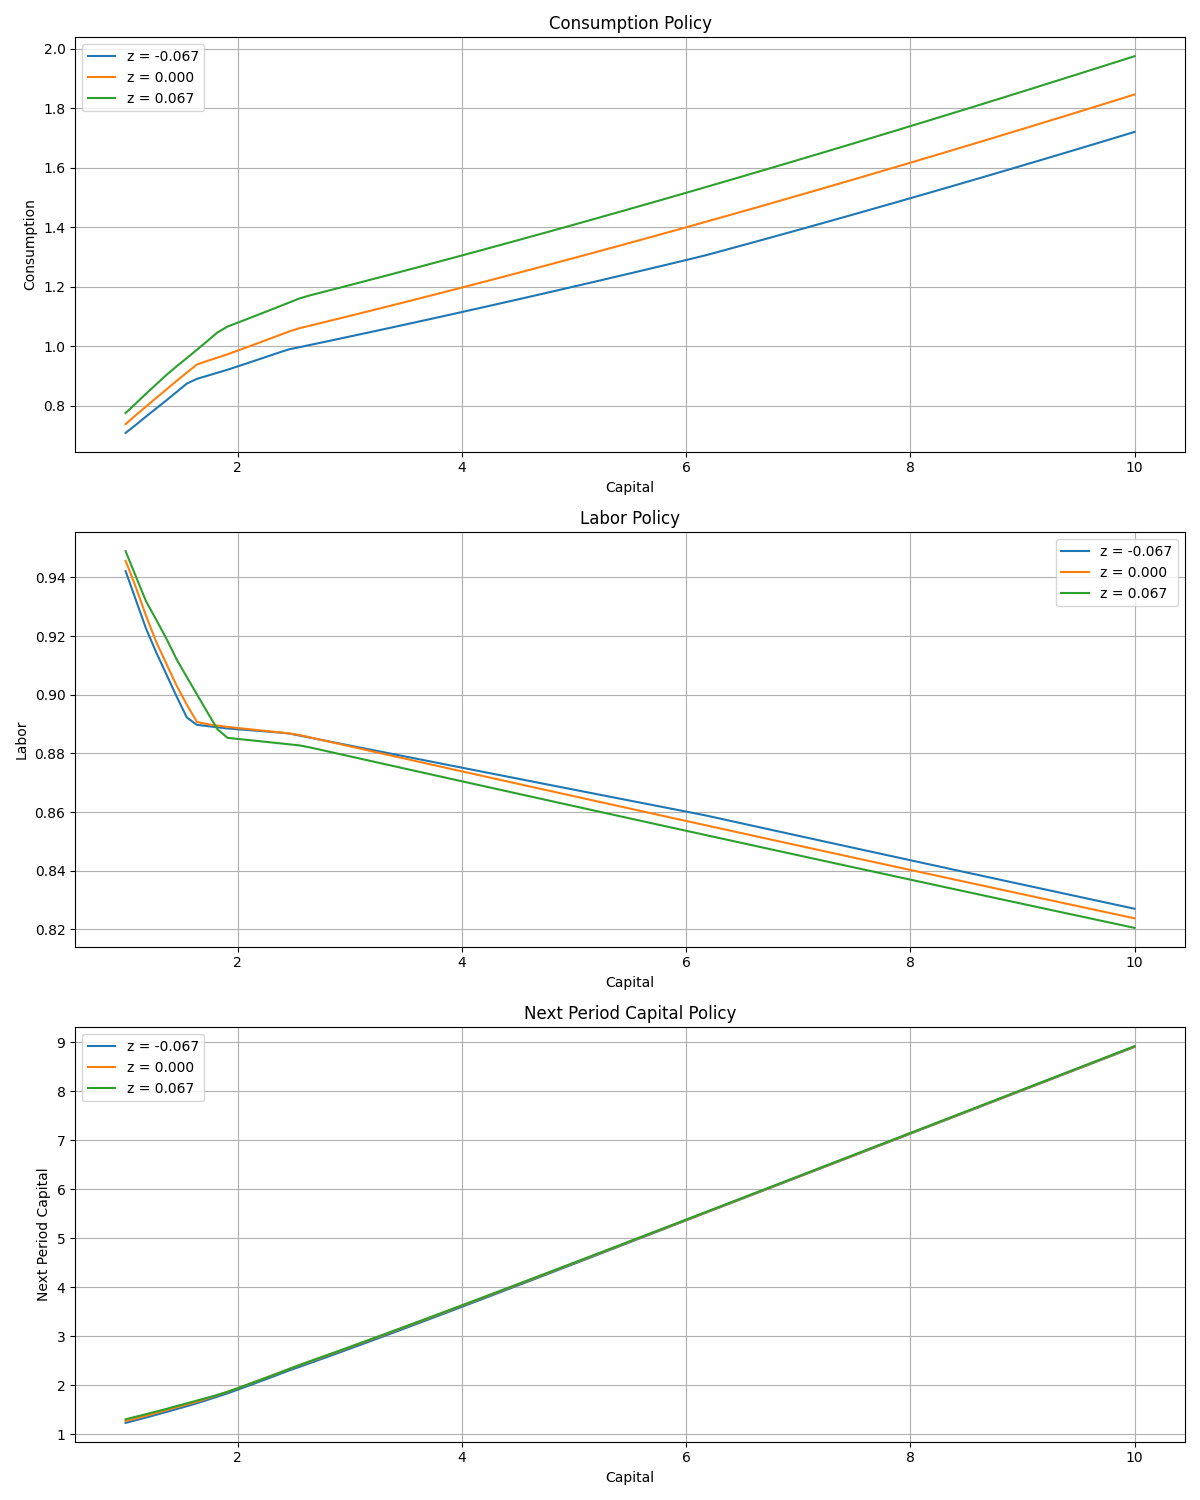
\includegraphics[width=\textwidth]{q4fin.png}
		\caption{Machine Learning Policy Functions}
	\end{figure}

\end{document}